\scanpage{40}
% archive foliation: 39
\diagram{\begin{tikzcd}
& X \arrow[d] & X\times_S S' \arrow[ul] \arrow[d] \\
S & T \arrow[l,"f"'] & \\
\unsure{S'|Z'} \arrow[uu] & S'\times_S T=T' \arrow[l] \arrow[u] \arrow[uur,dashed,bend right] &
\end{tikzcd}}
\diagram{\begin{tikzcd}
& X_s \arrow[d] & X'_{s'} \arrow[ul] \arrow[d] \\
s \arrow[r,dash] & T_s & \\
s' \arrow[r,dash] & T'_{s'} \arrow[u] \arrow[uur,dashed,bend right] &
\end{tikzcd}}
\figure{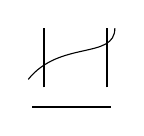
\begin{tikzpicture}[scale=.5]\draw (0,0)--(0,1.5);\draw (1.6,0)--(1.6,1.5);\draw (-.4,.2) .. controls (.4,1.2) and (1.8,.7) .. (1.8,1.5);\draw(-.3,-.5)--(1.7,-.5);\end{tikzpicture}}
\uline{Proposition 2} Supposons que $f_*(X/T)$ existe, et que pour tt $s\in S$, \deleted{toute} multisection de $X_s/T_s$ définie sur une extension finie \inserted{$k'$} [quelc] de $k(s)$, soit ``contenue'' dans un ouvert \deleted{\unsure{affine relatif|affine}} $U_i\otimes k'$ ($U_i$, \unsure{famille d'ouverts donnée|famille donnée}). Alors $f_*(X/T)$ est réunion des $f_{i*}(U_i/T)$ ($\unsure{f_i=f(U_i)|f_i=f\vert U_i}$).
\margin{\unsure{de finité}}
[On suppose $T$ et $X$ de type fini sur $S$]

En effet, \deleted{\unsure{on}} il suffit de montrer pour \deleted{\unsure{tout}} pt \deleted{fermé} de $f_*(X/T)$ que \unsure{$\exists i:\ \in f_{i*}(U_i/T)$}.
Un tel pt fermé est défini par un corps $K$ sur un $k(s)$, et une \inserted{multi}section définie sur $K$ de $X_s$ sur $T_s$. On peut le supposer \deleted{défini sur un} $K$ fini sur $k(s)$, à cause des hyp. de finitude \unsure{faites dans le|posées dans le} \deleted{\illegible{1}} premier cas. Il provient donc \unsure{---}.

\margin{\unsure{complète prop. 2}}
\deleted{\uuline{Corollaire}} \inserted{\uline{Proposition $2^{bis}$}} Supposons que les \inserted{multi}sections $X_s/T_s$ définies sur une extension finie (ou p. \unsure{quelconque}) $k'$ de $k(s)$ soient contenues dans un ouvert \deleted{\uline{affine}} \deleted{\unsure{relatif}} \inserted{d'}une famille $U_i$.
Supposons que les $f_{i*}(U_i/T)$ existent, alors il en est de $=$ de $f_*(X/T)$.
